\chapter{Popup Menu and Action Bar}

\section{Introduction}
...To be filled...

\section{Popup Menu}
\subsection{Create New Project}
\label{PMAB:createNewProject}
Create a new project from scratch. Perform the following steps:
\begin{enumerate}
	\item Create a new project having name ``\texttt{PopupMenuApp}''
	\item Select minimum API 16 : Android 4.1 (Jelly Bean).
	\item Select ``\texttt{Empty Activity}''
	\item Accept default values for activity and click finish. \\
\end{enumerate}

A popup or a drop down menu is a simple floating menu that you can display pretty much anywhere. It contains clickable items that you can interact with. This is a very useful feature when you don't want the user interface to be cluttered with buttons. Following example shows popup menus in action:

\begin{center}
	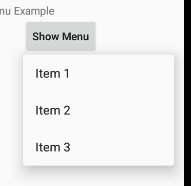
\includegraphics[scale=0.4]{chapters/ch07/images/37}
\end{center}

\vskip 4mm
To create a popup menu, there are three basic steps:
\begin{enumerate}
	\item Create a menu resource xml file. This will describe the items that the menu will have.
	\item Create a popup menu object and inflate the menu xml.
	\item Add an event listener that gets called whenever \textit{any} menu item or sub-item gets called.
\end{enumerate}

\subsection{Creating Menu Resource}
\label{PMAB:createingMenuResource}
Like other resources, the menu resource files reside in a special folder designated to its purpose, called the \texttt{menu} folder. To create a menu resource, go to the project panel and right click on the \texttt{res} folder. A popup menu opens up. Select ``New $\rightarrow$ Android resource file''. A dialog box opens up. Enter ``\texttt{my\_menu}'' as file name. Make sure that you select ``Menu'' from the ``Resource type'' drop down menu. Click OK.

A new xml resource file named ``\texttt{my\_menu.xml}'' will be created inside the \texttt{menu} folder:

\begin{center}
	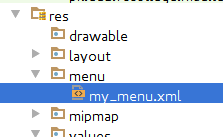
\includegraphics[scale=0.4]{chapters/ch07/images/38}
\end{center}

The way to add items in a menu is through \texttt{<item>} tag. Open up \texttt{my\_menu.xml} and add the following three items:

\begin{center}
	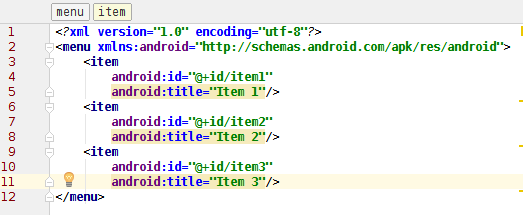
\includegraphics[scale=0.4]{chapters/ch07/images/39}
\end{center}

Actually, we can even nest menus within menus. Let's add two children under menu ``item 1'' (lines 6 to 14):

\begin{center}
	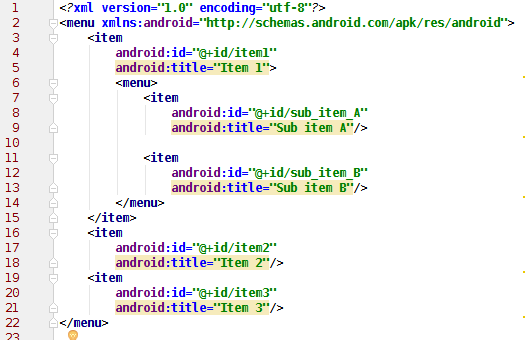
\includegraphics[scale=0.4]{chapters/ch07/images/40}
\end{center}

Now whenever the user selects ``item 1'', another sub-menu will popup with two items namely ``Sub item A'' and ``Sub item B''.

\begin{quote}
	``\textit{\underline{\textbf{IMPORTANT:}} You should \textbf{NEVER} hardcode the item titles. \textbf{ALWAYS} use string resources (by first defining them in the string resource file). In fact as an exercise, replace all the hardcoded menu titles with string resources.}''
\end{quote}

\subsection{Instantiating the Menu Object in Java}
Now that we've created a nice menu resource, it's time to actually create and display the menu in java code. Let's hook up the menu with say a button click (although you can hook it up with anything, even a finger tap on the screen!)

Open up \texttt{activity\_main.xml} and create a simple layout matching the following (it contains just one text view and a single button):

\begin{center}
	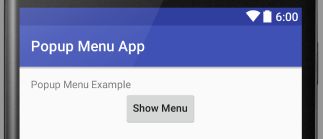
\includegraphics[scale=0.4]{chapters/ch07/images/41}
\end{center}

Hook up the button above to an event listener method called \texttt{btnClick}. Then inside this method, create a popup menu object, inflate the menu resource and finally display the menu:

\begin{center}
	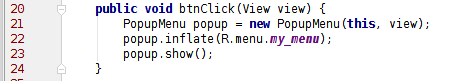
\includegraphics[scale=0.4]{chapters/ch07/images/42}
\end{center}

\begin{itemize}
	\item \textit{Line 21:} Instantiate a new \texttt{PopupMenu} object. The constructor takes two parameters. First one is the \texttt{context}. You can think of this as the parent of this menu. You can either use the \texttt{getApplicationContext} method to get the context or alternatively just pass in \texttt{this}.
	
	The second parameter is the ``anchor'' view. Popup will be displayed below this anchor if there is room. We want our anchor to be the button so we passed its reference. You can set ANY anchor on the layout you want.
	
	\item \textit{Line 22:} Inflate the menu resource xml file and create actual menu to be rendered.
	
	\item \textit{Line 23:} Finally display the menu on the screen.
\end{itemize}

Run the app on a device. When you click the button, you should see the menu being popup having all the items and child items that we specified in the menu xml resource. You can click on the items and browse sub items but they do nothing yet. We will make them come alive in the next section.

\subsection{Adding Event Listener to the Menu}
\label{PMAB:addEventListenerToMenu}
You need to add event listeners if you want to register user click events. Just like buttons there are multiple ways to add listeners to the menus. More details on how to attach listeners to the buttons through java code are given in lecture 5 section 2.3. The procedure for the menus is almost exactly the same. \\

Let's add the listeners using an anonymous inner class. In the \texttt{btnClick} method, just after where popup is being shown, add the following code (lines 24 to 33):

\begin{center}
	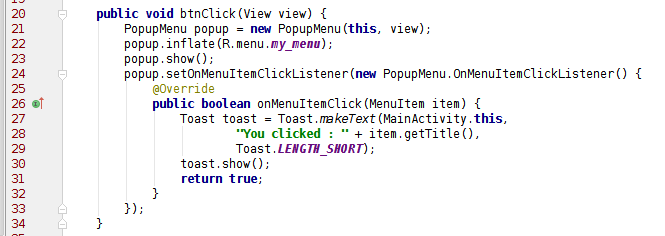
\includegraphics[scale=0.4]{chapters/ch07/images/43}
\end{center}

Don't forget to put a ``\texttt{;}'' at the end of line 33.

This piece of code should look very familiar to you by now. Run it on a device and see how clicking on any menu item displays a toast on the screen. \\

Instead of anonymous inner classes, you can also use the alternative method (as explained in detail in Lecture 5 section 2.3.3) to add menu event listeners. \\

For more information about popup menus visit the link \href{https://developer.android.com/reference/android/widget/PopupMenu.html}{here}.

\subsection{Exercise}
Study code listed in section \ref{PMAB:addEventListenerToMenu} in detail and find our how everything is working including the details about what \href{https://developer.android.com/reference/android/widget/PopupMenu.OnMenuItemClickListener.html}{\texttt{PopupMenu.OnMenuItemClickListener}} and \href{https://developer.android.com/reference/android/view/MenuItem.html}{\texttt{MenuItem}} interfaces are.



\section{The Action bar}
The action bar (also known as toolbar on newer systems) is located near the top edge of the app. It is a very flexible component that you can utilize to make great apps:

\begin{center}
	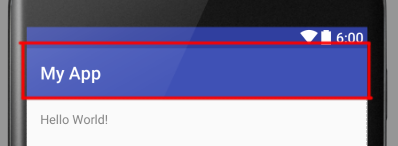
\includegraphics[scale=0.4]{chapters/ch07/images/27}
\end{center}

Toolbar is a relatively new addition introduced in OS version 5.0, API level 21 (Lollipop). Earlier it was known as the ``App bar'' or even ``Action bar''. Toolbar, app bar and action bar are very similar widgets, very minor differences. In fact the toolbar is built upon the app bar. 

We can still use the toolbar on older OS versions such as API level 16 (Jelly Bean). Fortunately for us the android provides libraries such as ``\texttt{AppCompat}''. This library allow even the older versions to display toolbar like the one in the latest OS version 7.0! \\

Create a new project from scratch as shown in section \ref{PMAB:createNewProject} and name it anything you like. For this section we assume the name \texttt{}. \\

If you open up \texttt{MainActivity.java} you will observe that the \texttt{MainActivity} class has been extended from \texttt{AppCompatActivity} instead of just \texttt{Activity}. The \texttt{AppCompatActivity} class tries to provide functionality of the newer systems on older devices. Since we are just touching the subject without going into advanced features, we will be using both terms i.e \texttt{Toolbar} and \texttt{App bar} interchangeably. 

\subsection{Hiding the Toolbar}

Let's hide the toolbar (action bar). If you haven't already, open up \texttt{MainActivity.java} and add the following lines (15, 16):

\begin{center}
	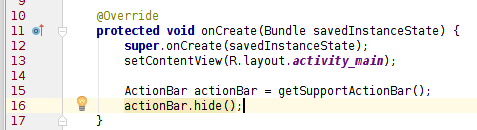
\includegraphics[scale=0.4]{chapters/ch07/images/28}
\end{center}

\begin{itemize}
	\item \textit{Line 15:} Get reference to the action bar. Since we are working on an older OS (API 16) we need to call the support library method \texttt{getSupportActionBar} to get the reference to our action bar (on more recent OS such as 5.0 you can just call \texttt{getActionBar}).
	
	\item \textit{Line 16:} Hide the action bar.
\end{itemize}

When you run the app on a device you'll notice that the action bar is now gone:

\begin{center}
	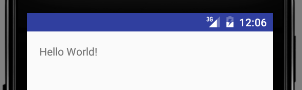
\includegraphics[scale=0.4]{chapters/ch07/images/29}
\end{center}

\vskip 4mm
\textit{Great! Now you know how to hide the action bar, delete lines 15 and 16 so that we can proceed to the next section.}

\subsection{Attaching Menu to Action Bar}
We can also add a reasonably complex menu to the action bar. Adding menu to the action bar is a multi-step process. First you need to create a menu resource (which is an XML file). Then inflate the menu resource XML into a view group. Finally attach event listeners to handle user interaction.

\subsubsection{Creating Menu Resource}
Following the steps mentioned in section \ref{PMAB:createingMenuResource}, create a new menu resource XML file. You are free to use the menu XML file given in section \ref{PMAB:createingMenuResource}, or if you prefer you can create your own menu items from scratch. For the following sections we assume that you've named your menu XML file as ``\texttt{my\_menu.xml}''.

\subsubsection{Inflating the Menu}
Next step is to inflate the menu. For the menu to show up as the app starts we need to override the \texttt{Activity} class's \href{https://developer.android.com/reference/android/app/Activity.html#onCreateOptionsMenu(android.view.Menu)}{\texttt{onCreateOptionsMenu}} method. This method is called \textit{only once} when the menu is about to be displayed (or when the menu is invalidated for some reason). Open up ``\texttt{MainActivity.java}''. Override this method in the \texttt{MainActivity} class and add the code that inflates the menu:

\begin{center}
	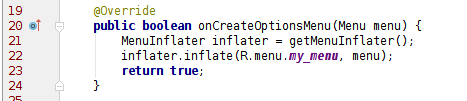
\includegraphics[scale=0.4]{chapters/ch07/images/44}
\end{center}

Let's review the code line by line:

\begin{itemize}
	\item \textit{Line 20}: The overridden method that gets called only the first time the menu is about to be displayed. It provides access to the menu object through its parameters. 
	
	\item \textit{Line 21}: Get the \href{https://developer.android.com/reference/android/view/MenuInflater.html}{\texttt{MenuInflater}} reference. Menu inflater is very similar to the layout inflater. 

	\item \textit{Line 22}: Finally inflate the menu resource inside \texttt{menu} object using the \texttt{MenuInflater}'s ``\texttt{inflate}'' method. The \texttt{inflate} method two parameters. The first parameter is the id of the menu resource. Second parameter is the menu object inside which menu resource is to be inflated.
\end{itemize}

Now if you run the app on a device, you will see three vertical dots on the right side of the action bar:

\begin{center}
	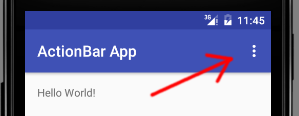
\includegraphics[scale=0.4]{chapters/ch07/images/45}
\end{center}

This shows that our menu has been successfully created and attached to the action bar. If you tap on the dots, a menu opens up containing all the items that we specified in the XML resource:

\begin{center}
	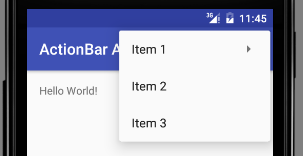
\includegraphics[scale=0.4]{chapters/ch07/images/46}
\end{center}

Right now you can navigate through the menu but clicking on any item won't do anything. We need to attach event listeners to the menu as we will see in the next section.

\subsubsection{Handling Menu Events}
To handle menu events you need to override the \texttt{Activity}'s ``\href{https://developer.android.com/reference/android/app/Activity.html#onOptionsItemSelected(android.view.MenuItem)}{\texttt{onOptionsItemSelected}}'' method. Whenever you click on any menu item, this method will be called. Open up \texttt{MainActivity.java} and override the following method in \texttt{MainActivity} class:

\begin{center}
	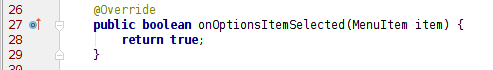
\includegraphics[scale=0.4]{chapters/ch07/images/47}
\end{center}

Let's display the name of the item clicked by the user. Add following line to the code (line 28):

\begin{center}
	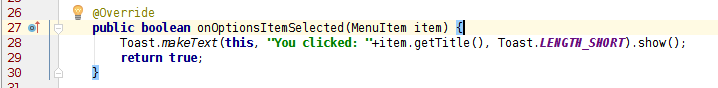
\includegraphics[scale=0.4]{chapters/ch07/images/48}
\end{center}

We are just getting text label of the clicked item and displaying that string using a toast. Run the app on a device and see if it works properly. \\

There are two ways to identify the exact item that was clicked. One is to match the text labels of the items and check which one was selected. Go to the \texttt{onOptionsItemSelected} method modify it as follows:

\begin{center}
	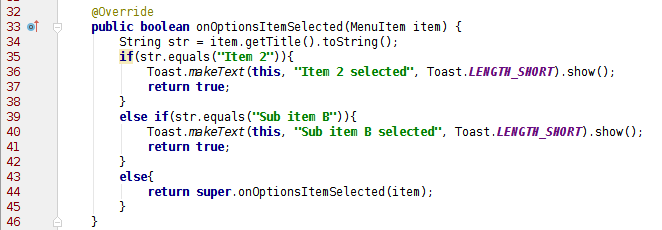
\includegraphics[scale=0.4]{chapters/ch07/images/49}
\end{center}

Let's look at it line by line:

\begin{itemize}
	\item \textit{Line 33:} Method signature. Note the parameter \texttt{item} of type \texttt{MenuItem}. This is the reference of the menu item that was clicked by the user.
	
	\item \textit{Line 34:} Get the text label of that menu item and convert it into java \texttt{String}.
	
	\item \textit{Lines 35 to 42:} Here you can compare the item labels with hard coded strings. You can add multiple \texttt{if/else} clauses in case if you need to manage other items. In case of a match (line 36 or 40) simply display a toast and return \texttt{true}.
	
	\item \textit{Line 44:} In case if the desired string was not matched then return the super class's \texttt{onOptionsItemSelected} to properly handle the missing case. 
	
	\underline{\textbf{Important:}} If you try to call \texttt{onOptionsItemSelected} without the super keyword then this will result in an infinite recursion and your app will freeze. \\
\end{itemize}

However please note that multiple menu items can have the same label, for instance one item on the main menu and the other item can be hidden deep inside sub-sub menus. Hence checking the identity of a menu item via the string label is not a good idea. Use the \texttt{id} instead because the \texttt{id}s are guaranteed to be unique. Take a look at the \texttt{id}s we specified for each of the items in \texttt{my\_menu.xml} menu resource file. If not already, open up \texttt{MainActivity.java} and go to \texttt{onOptionsItemSelected}. Modify it as follows. This time we are going to match the \texttt{id}s:

\begin{center}
	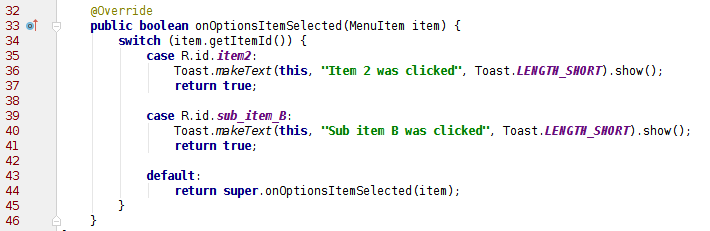
\includegraphics[scale=0.4]{chapters/ch07/images/50}
\end{center}

\subsection{Placing Menu Item on Action Bar}
There are various ways you can display the menu items on an action bar. Uptill now all of the items were hidden inside a menu attached to the three dots on the right. However you can display some of the items on the action bar itself, depending on the space available.\\

We will use the menu resource xml from section \ref{PMAB:createingMenuResource}. Open up \texttt{my\_menu.xml}. In the \texttt{<Item>} element having title ``Item 2'', add an attribute called ``\texttt{app:showAsAction}'' and set it to \texttt{always} (shown in line 19 below):

\begin{center}
	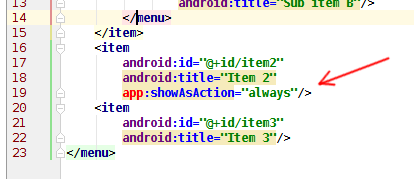
\includegraphics[scale=0.4]{chapters/ch07/images/51}
\end{center}

If you look closely at the xml file, almost all of the attributes are preceded by ``\texttt{android:}''. This is the namespace containing all of the attributes available in the current android OS version. The keyword ``\texttt{app:}'' before \texttt{showAsAction} attribute is the global namespace which includes extra attributes added via an external library (\texttt{appcompat}) that are not available in the current OS version. 

To simply put toolbar is a new feature not available on old OS versions. We need to use the ``\texttt{app:}'' on older systems to support newer features. On newer OS such as Marshmallow or Nougat you can simple use the \texttt{android:} because these recent android versions contain all the attributes that we want to use.

Notice that the \texttt{app:} keyword in line 19 is highlighted in red. Move your keyboard cursor on top of \texttt{app:}. A simple callout will appear asking you to include the pre-requisites by pressing ``\texttt{Alt+Enter}'':

\begin{center}
	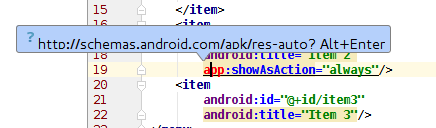
\includegraphics[scale=0.4]{chapters/ch07/images/52}
\end{center}

By pressing \texttt{Alt+Enter} android studio will add essential pre-requisites for the app namespace inside the menu element. Here you can see that it defined a new \texttt{app} attribute for out use in line 3:

\begin{center}
	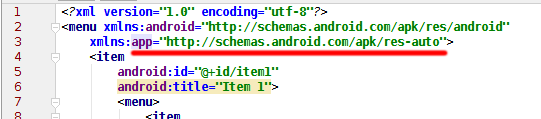
\includegraphics[scale=0.4]{chapters/ch07/images/53}
\end{center}

Alright, fine, but what does ``\texttt{app:showAsAction}'' attribute do? Well, if it is set to ``\texttt{always}'' then that menu item will ALWAYS be shown on the main action bar. In this case we've set this field to always for menu ``item 2''. Run the app and you'll see ``item 2'' now being displayed on the action bar:

\begin{center}
	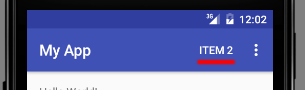
\includegraphics[scale=0.4]{chapters/ch07/images/54}
\end{center}

If you click it you should see a toast pop up on the screen. If you click the dots on the right side of the action bar to open up our menu, you will notice that item 2 is no longer listed there, because it is now displayed on the action bar. 

Other values for the ``\texttt{showAsAction}'' that you can set are \texttt{never}, \texttt{ifRoom}, \texttt{withText}, \texttt{collapseActionView}. \textit{It is left up to you as an exercise to figure out the exact function of each of these.}

\subsection{Adding Pictures to the Menu Items}
You can also add pictures or icons next to the items to make them more interesting. Let's first create some graphics resources fir menu ``Item 2''. \\

Open up android asset generator (\texttt{File}$\rightarrow$\texttt{New}$\rightarrow$\texttt{Image Asset}). Refer to section \ref{ITS:changingLauncherIconThroughAndroidStudio} for detailed introduction to this tool. Select ``''

\begin{center}
	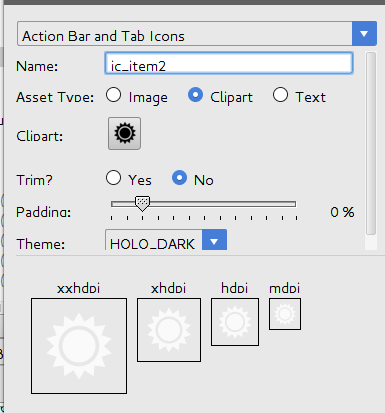
\includegraphics[scale=0.4]{chapters/ch07/images/55}
\end{center}

Select ``Action Bar and Tab Icons'' from the drop down menu. In the name field give appropriate name relating to the menu item that you are creating the graphic for. Set the ``Asset Type'' to ``Clipart'' (you can also use external images but for now let's keep it simple). Select the these to ``Holo dark'' because we want to show light colored icons on our dark colored action bar. Finally press \texttt{OK} to generate the set of different resolution graphics. You can view these in corresponding \texttt{drawable} folders.

\begin{quote}
	\textit{\textbf{Warning:} The name of the icon should only contain small case a-z, digits 0-9 and underscores. Any other character or even capital letters in the graphic file name will result in a compiler error!}
\end{quote}

Open up \texttt{my\_menu.xml} and go to Item 2's element. Add an attribute ``\texttt{android:icon}'' and give it the \texttt{id} of our graphics resource \texttt{ic\_item2}:

\begin{center}
	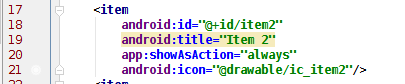
\includegraphics[scale=0.4]{chapters/ch07/images/56}
\end{center}

Run the app on a device and you will see something like this:

\begin{center}
	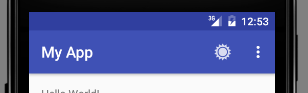
\includegraphics[scale=0.4]{chapters/ch07/images/57}
\end{center}

Read more about action bar and its design guide \href{https://developer.android.com/design/patterns/actionbar.html}{here}.

\section{Contextual Menus}

\section{Menu Groups}